\apendice{Especificación de diseño} \label{ch:design}

\section{Introducción} \label{sec:design-intro}
Tras recoger las especificaciones de los requisitos del \sw{} se 
puede comenzar con la especificación del diseño. Este apéndice detalla
las soluciones tomadas respecto al diseño del \sw{}.

Con el diseño del \sw{} se trata de dar respuesta a cuestiones relativas a los
datos, y su representación; las división lógica en módulos, y su funcionamiento
interno; y como estructurar el \sw{} arquitectónicamente.

\subsection{Ámbito del \sw{}} \label{sec:design-ambito}
El \sw{} a desarrollar debe permitir a un usuario operar con un
sistema empotrado de forma remota a través de una aplicación web. Al ser
entidades tan diferenciadas, tanto el sistema empotrado como la aplicación web
tienen que contar con \sw{} propio y específico a cada plataforma.

El \sw{} del sistema empotrado tiene que residir en el propio sistema. Con su
ejecución se pretende actuar sobre el \hw{} habilitado a tal fin.

En cuanto al \sw{} de la aplicación web, ejecutado en un servidor de aplicaciones, va a
servir como interfaz de usuario frente al sistema empotrado que le va a permitir
ordenar la ejecución de las funciones del sistema empotrado.



\section{Diseño de datos} \label{sec:design-datos}
Para que la aplicación web pueda ordenar al sistema empotrado actuar de una
determinada manera se precisa de la transmisión de unos comandos concretos. En
consecuencia, se tiene que definir la estructura de los comandos para que ambos
\extranjerismo{softwares} sean capaces de entenderse.


\subsection{Transferencia de los comandos} \label{sec:design-transferencia}
Los comandos van a ser transferidos usando el protocolo Transmission Control
Protocol (TCP). El protocolo está orientado a la conexión y se encarga de
establecerla la comunicación mediante unos mensajes de sincronización (SYN) y
reconocimiento (ACK), como se puede ver en \ref{fig:tcp}.

\begin{figure}[!h]
  \centering
  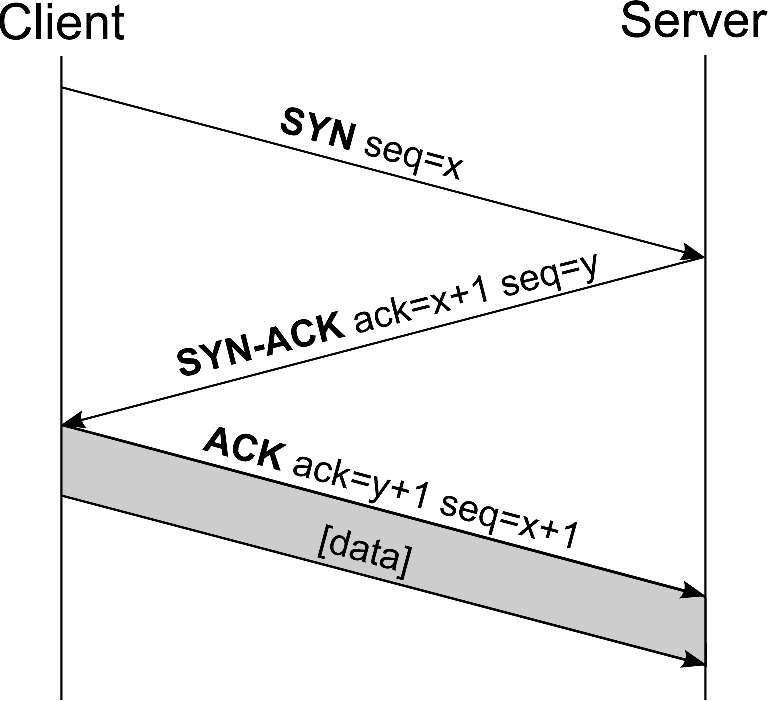
\includegraphics[width=0.6\textwidth]{tcp}
  \caption{Conexión TCP \cite{webpage:tcp-handshake}} \label{fig:tcp}
\end{figure}

Aprovechando que el protocolo TCP se encarga establecer una conexión fiable,
se delega en él el establecimiento de la conexión y los comandos serán enviados
después encapsulados dentro de segmentos TCP.


\subsection{Comando LED} \label{sec:design-datos-led}
Con este comando se indica al sistema empotrado que muestre una luz con el color
indicado. Hay un LED para cada uno de los tres colores primarios: rojo, verde y
azul. Aunque los LED pueden encenderse individualmente, encendiéndolos
simultáneamente se pueden combinar los colores primarios y generar otros
nuevos. Los colores obtenidos por adición son el cian, magenta, amarillo y
blanco. Además, debe ser posible que los LED se apaguen y dejen de iluminar.

Para conseguir lo anterior, el nombre del comando refleja la alusión a los LED
RGB. El comando se acompaña de un argumento que especifica el color concreto a
iluminar. Para ayudar a diferenciar el comando del argumento se ubica un carácter
separador.

\tablaSmallSinColores{Comando LED}{l c c c c}{comando-led}
{\multicolumn{1}{l}{Color} & Comando & Separador & Argumento & Comando resultante\\}
{
  Rojo     & led & : & r & led:r \\
  Verde    & led & : & g & led:g \\
  Azul     & led & : & b & led:b \\
  Cian     & led & : & c & led:c \\
  Magenta  & led & : & m & led:m \\
  Amarillo & led & : & y & led:y \\
  Blanco   & led & : & w & led:w \\
  No color & led & : & o & led:o \\
}


\subsection{Comando MSG} \label{sec:design-datos-msg}
Este comando indica al sistema empotrado que muestre una cadena de caracteres
en la pantalla LCD. Como la pantalla tiene dos líneas, se necesita indicar
la línea donde mostrar el texto.

El nombre del comando refleja que trata con los mensajes de texto. El comando
se acompaña de un argumento que especifica la línea donde escribir la cadena de
caracteres. Después se añade otro argumento con la cadena de caracteres a
mostrar. Como en el resto de comandos, entre el comando y cada uno de los
argumentos se ubica un carácter separador. 

\tablaSmallSinColores{Comando MSG}{l c c c c c c}{comando-msg}
{\multicolumn{1}{l}{Línea} & Comando & S. & Arg. 1 & S.
                           & Arg. 2 & Comando resultante\\}
{
  1\textsuperscript{a} línea & msg & : & 0 & : & <chars> & msg:0:<chars>\\
  2\textsuperscript{a} línea & msg & : & 1 & : & <chars> & msg:1:<chars>\\
}


\subsection{Comando PWM} \label{sec:design-datos-pwm}
Este comando indica al sistema empotrado que regule la intensidad del brillo de
los LED compatibles con PWM. El sistema empotrado cuenta con 4 LED regulables
por lo que es necesario identificar cual de ellos hay que regular.

El nombre del comando refleja que se van a utilizar los LED PWM. Como hay 4 LED
hace falta un argumento que permita seleccionar el LED a regular. Para indicar
la intensidad se añade otro argumento con el valor nuevo, entre 0 y 100.
De nuevo, entre el comando y cada uno de los argumentos se ubica un carácter
separador. Por último, se añade de nuevo un carácter con el color de LED para
indicar al sistema empotrado que ha finalizado el valor numérico. 

\tablaSmallSinColores{Comando PWM}{l c c c c c c c}{comando-pwm}
{\multicolumn{1}{l}{LED} & Comando & S. & Arg. 1 & S.
                           & Arg. 2 & Fin & Cmd. resultante\\}
{
  Blanco   & pwm & : & w & : & <0-100> & w & pwm:w:<0-100>w \\
  Verde    & pwm & : & g & : & <0-100> & g & pwm:g:<0-100>g \\
  Amarillo & pwm & : & y & : & <0-100> & a & pwm:y:<0-100>a \\
  Rojo     & pwm & : & r & : & <0-100> & r & pwm:r:<0-100>r \\
}



\section{Diseño arquitectónico} \label{sec:arch}
La arquitectura de un \sw{} se describe en el estándar IEEE 42010-2011
\cite{webpage:ieee42010-2011} como  los ``conceptos fundamentales o propiedades
de un sistema en su entorno encarnados por sus elementos, relaciones, y en los
principios de su diseño y evolución.''

Así pues, como los entornos del \sw{} del sistema empotrado y de la aplicación
web están tan diferenciados, se opta por usar estilos arquitectónicos diferentes
y adaptados a cada \sw{}.

\subsection{Diseño arquitectónico del SE} \label{sec:arch-se}
Los sistemas empotrados se relacionan con el entorno en el que se encuentran
mediante actuadores y sensores, y dependiendo de su finalidad, con
restricciones de tiempo real. La organización del \sw{} debe ajustarse a estas
realidades.

En sistemas sistemas simples sin restricciones de tiempo se puede organizar
el \sw{} de forma simple. En cambio, cuando las tareas de un sistema empotrado
tienen que responder rápidamente a eventos con restricciones de tiempo se hace
necesario organizar el \sw{} de forma más compleja.

En un sistema empotrado sin restricciones se podría utilizar la arquitectura
del \sw{} más simple conocida como Round Robin. Las tareas del sistema empotrado
se ejecutan dentro de un bucle principal, en ellas se examina el estado \hw{} y
de ser necesario se realiza el tratamiento correspondiente. Una vez terminada
una tarea, se ejecuta la siguiente, y al completar la última se vuelve a empezar
el ciclo con la primera de todas.

\imagenalto{arch_rr}{Tareas en bucle infinito}{!h}{0.5}

Para no tener que estar sondeando constantemente el \hw{}, se puede mejorar la 
arquitectura anterior incluyendo interrupciones. Estas señales permiten indicar
al sistema empotrado cuando ha ocurrido un evento y lo libera del sondeo
constante.

Si bien ambas arquitecturas serían factibles de aplicar al sistema empotrado,
con intención de dar respuesta al requisito no funcional sobre el rendimiento
y respuesta del sistema se va a usar una arquitectura basada en un Sistema
operativo en tiempo real (RTOS).

La decisión se fundamenta en la flexibilidad y el tiempo de respuesta que el
RTOS es capaz de proporcionar. Cada función del sistema se implementa dentro de
una tarea individual con una determinada prioridad. El RTOS se encarga de 
planificar el orden de ejecución de las tareas en base a la prioridad de cada
de ellas. 

Por lo tanto, una tarea con prioridad alta, porque necesita un tiempo
de respuesta estricto, es ejecutada antes que las demás. Más aún, se puede
configurar el RTOS para que desaloje una tarea de menor prioridad y pase a
ejecutar una de mayor prioridad.

\begin{figure}[!h]
  \centering
  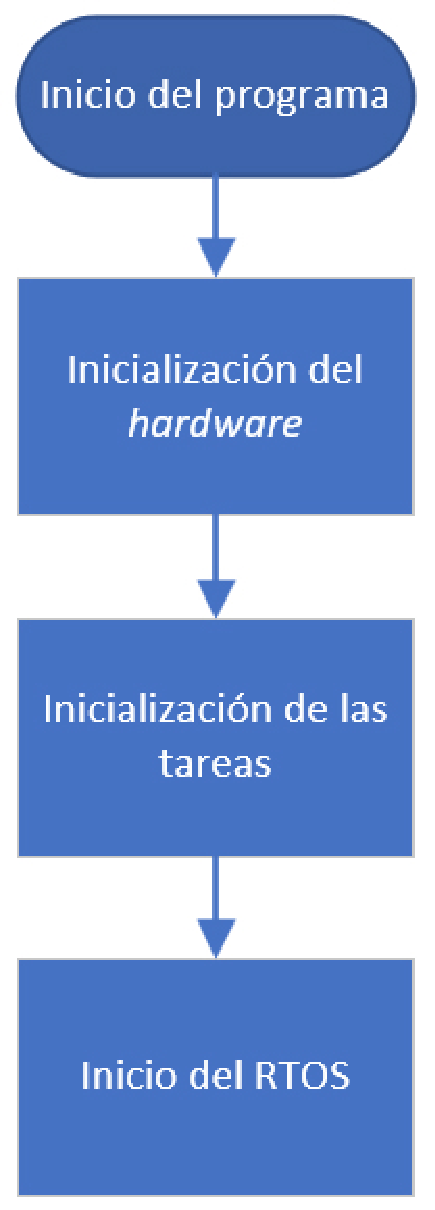
\includegraphics[height=0.5\textheight]{arch_bucle}
  \caption{Bucle principal del \sw{}} \label{fig:bucle}
\end{figure}

\begin{figure}[!h]
  \centering
  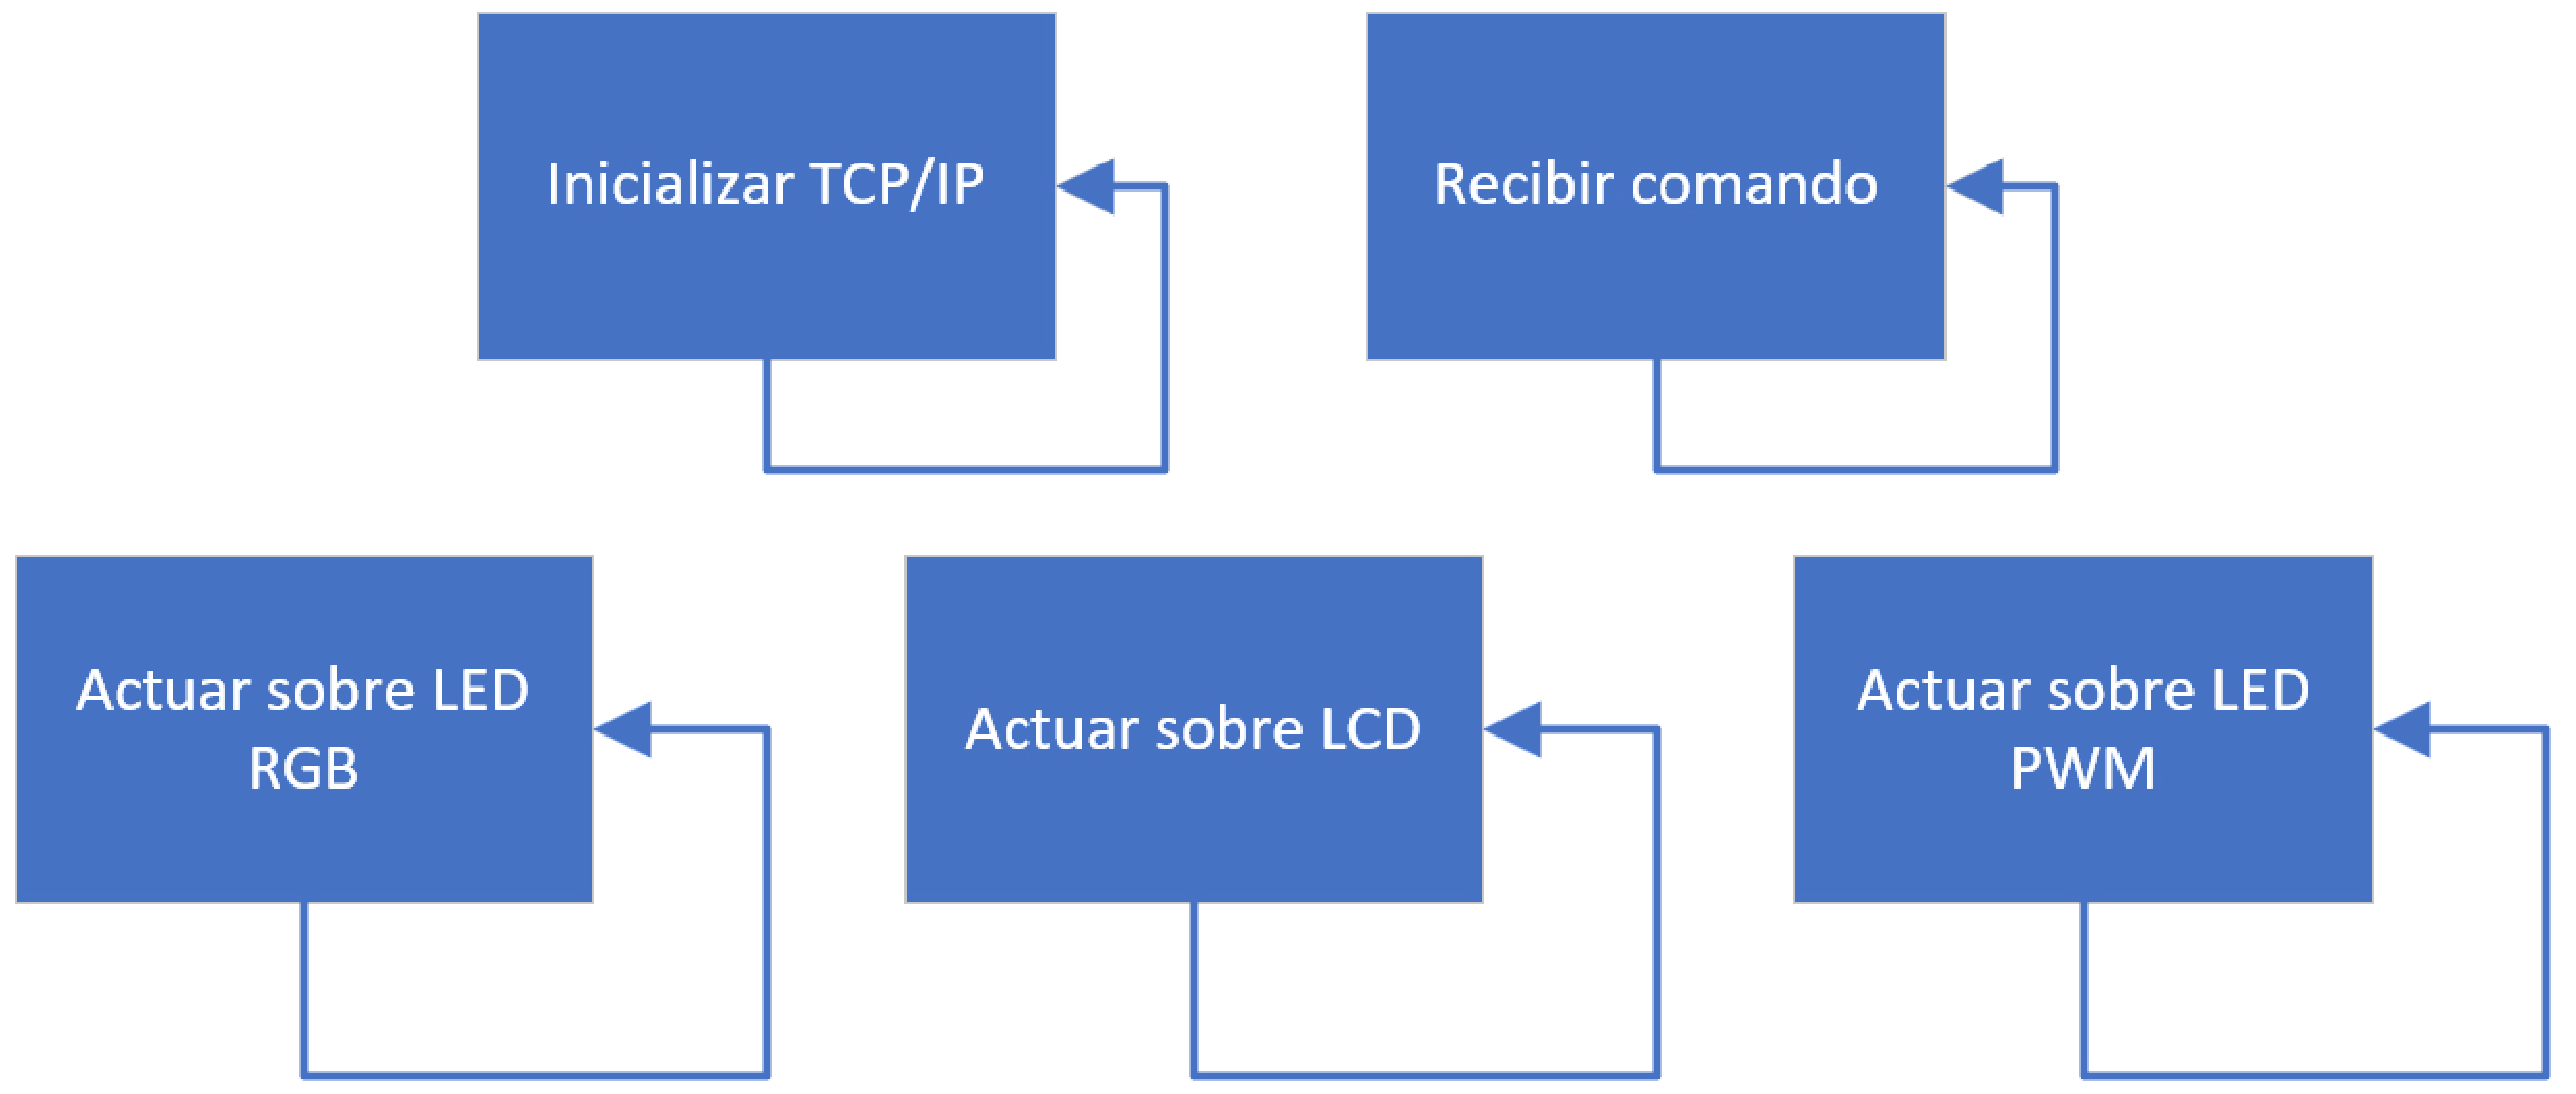
\includegraphics[width=0.6\textheight]{arch_tareas}
  \caption{Tareas para el RTOS} \label{fig:tareas}
\end{figure}

Con las tareas \ref{fig:tareas} se da respuesta a los casos de usos planteados
para el sistema empotrado durante la especificación de los requisitos del \sw{}.
Gracias la flexibilidad que aporta esta solución se podrían añadir o remover
funciones rápidamente. Por ejemplo, bastaría con agregarlas o quitarlas del 
RTOS durante la inicialización \ref{fig:bucle}.


\subsection{Diseño arquitectónico de la aplicación web} \label{sec:arch-aw}
Por lo que se refiere al \sw{} de aplicación web, representa un cambio de
contexto completo. La aplicación se encuentra alojada en un servidor de
aplicaciones que permite al usuario acceder a la interfaz web desde un
navegador web cualquiera.

La tecnología a utilizar en conjunción con el servidor de aplicaciones es
JavaServer Faces (JSF) \cite{webpage:jsf}. Su especificación concreta su
propósito para construir aplicaciones web e interfaces de usuarios basadas
en componentes. Cada componente de \sw{} sirve para encapsular un conjunto
de funciones o datos estrechamente relacionados.

Además, JSF utiliza el patrón de arquitectura Modelo-Vista-Controlador (MVC).
Este patrón separa la lógica de la aplicación en tres componentes diferenciados.
Con la separación se impulsa el desarrollo modular, facilitando la colaboración
y la reutilización durante el desarrollo.

Los tres componentes de MVC son:
\begin{description}
  \item[Modelo:] Define los datos y su estructura empleados por la aplicación.
  Si los datos se modifican, la vista se actualiza para reflejar los cambios.
  \item[Vista:] Define la interfaz y como se muestran los datos al usuario
  en ella.
  \item[Controlador:] Contiene la lógica responsable de manipular el modelo
  en función de las acciones del usuario.
\end{description}

\imagenancho{arch_mvc}{Relación entre MVC y el usuario}{!h}{0.8}

\subsubsection{Diseño del modelo} \label{sec:arch-modelo}
En JSF el modelo se define mediante \extranjerismo{beans}. Los
\extranjerismo{beans} se crean con clases Java. Están compuestos por una
conjunto de atributos y sus correspondientes métodos 
\extranjerismo{getters} y \extranjerismo{setters}.

Así pues, el valor de un atributo, también llamado propiedad, se consulta con
su correspondiente método \extranjerismo{get} y se puede actualizar con su
método \extranjerismo{set}.

\subsubsection{Diseño de la vista} \label{sec:arch-vista}
En JSF la vista se define mediante ficheros escritos en Extensible HyperText
Markup Language (XHTML) que incluyen etiquetas especiales para añadir
componentes específicos de JSF. Posteriormente, el código de los ficheros XHTML
es traducido a código Hypertext Markup Language (HTML) interpretable por los
navegadores web.

La conexión entre la interfaz y el resto de la aplicación se realiza con ayuda
del Lenguaje de Expresiones de JSF (EL). Con estas expresiones se enlazan los
componentes de la interfaz con las propiedades de los \extranjerismo{beans}.

\subsubsection{Diseño del controlador} \label{sec:arch-ctl}
En JSF el controlador se puede definir con \extranjerismo{beans} al igual
que en el modelo \ref{sec:arch-modelo}. Pero a diferencia de los
\extranjerismo{beans} del modelo, los \extranjerismo{beans} del controlador
cuentan con los métodos necesarios para realizar la lógica de negocio
requerida por la aplicación.


\subsection{Diseño conjunto del sistema} \label{sec:design-comp}

\imagenancho{componentes}{Diagrama de componentes del sistema}{!h}{1}


\subsection{Diagramas de clases} \label{sec:design-comp}

\imagenancho{pkg-controller}{Diagrama de clases de los paquetes
\extranjerismo{controller} y \extranjerismo{controller.network}}{H}{0.9}

\imagenalto{pkg-model}{Diagrama de clases del paquete
\extranjerismo{model}}{H}{0.3}


\subsection{Diseño de la interfaz} \label{sec:design-iface}
Para que el usuario pueda controlar el sistema empotrado, la aplicación web
pone su disposición una interfaz web. En una sola página el usuario puede
ver las funciones disponibles y operar con ellas.

En primer lugar la interfaz tiene que permitir que el usuario introduzca
los datos de conexión con el sistema empotrado.

\imagenancho{panel_datos}{Introducción de datos}{!h}{0.9}

Una vez establecidos los datos se muestran unos paneles con las funciones
disponibles.

Con unos botones se puede escoger el color iluminado por los LED RGB.

\imagenancho{panel_led}{Panel para cambiar el color de los LED RGB}{!h}{0.9}

En unos cuadros de texto, el usuario puede introducir un mensaje y pulsando
un botón lo puede enviar.
\imagenancho{panel_msg}{Panel para enviar un texto al LCD}{!h}{0.9}

\clearpage

Con unos controles deslizantes, el usuario puede cambiar la intensidad del brillo
de los LED regulados por PWM.
\imagenancho{panel_pwm}{Panel para regular el brillo de los LED PWM}{!h}{0.9}

\clearpage

La interfaz completa se construye según lo definido en el siguiente diseño.

\begin{figure}[H]
  \centering
  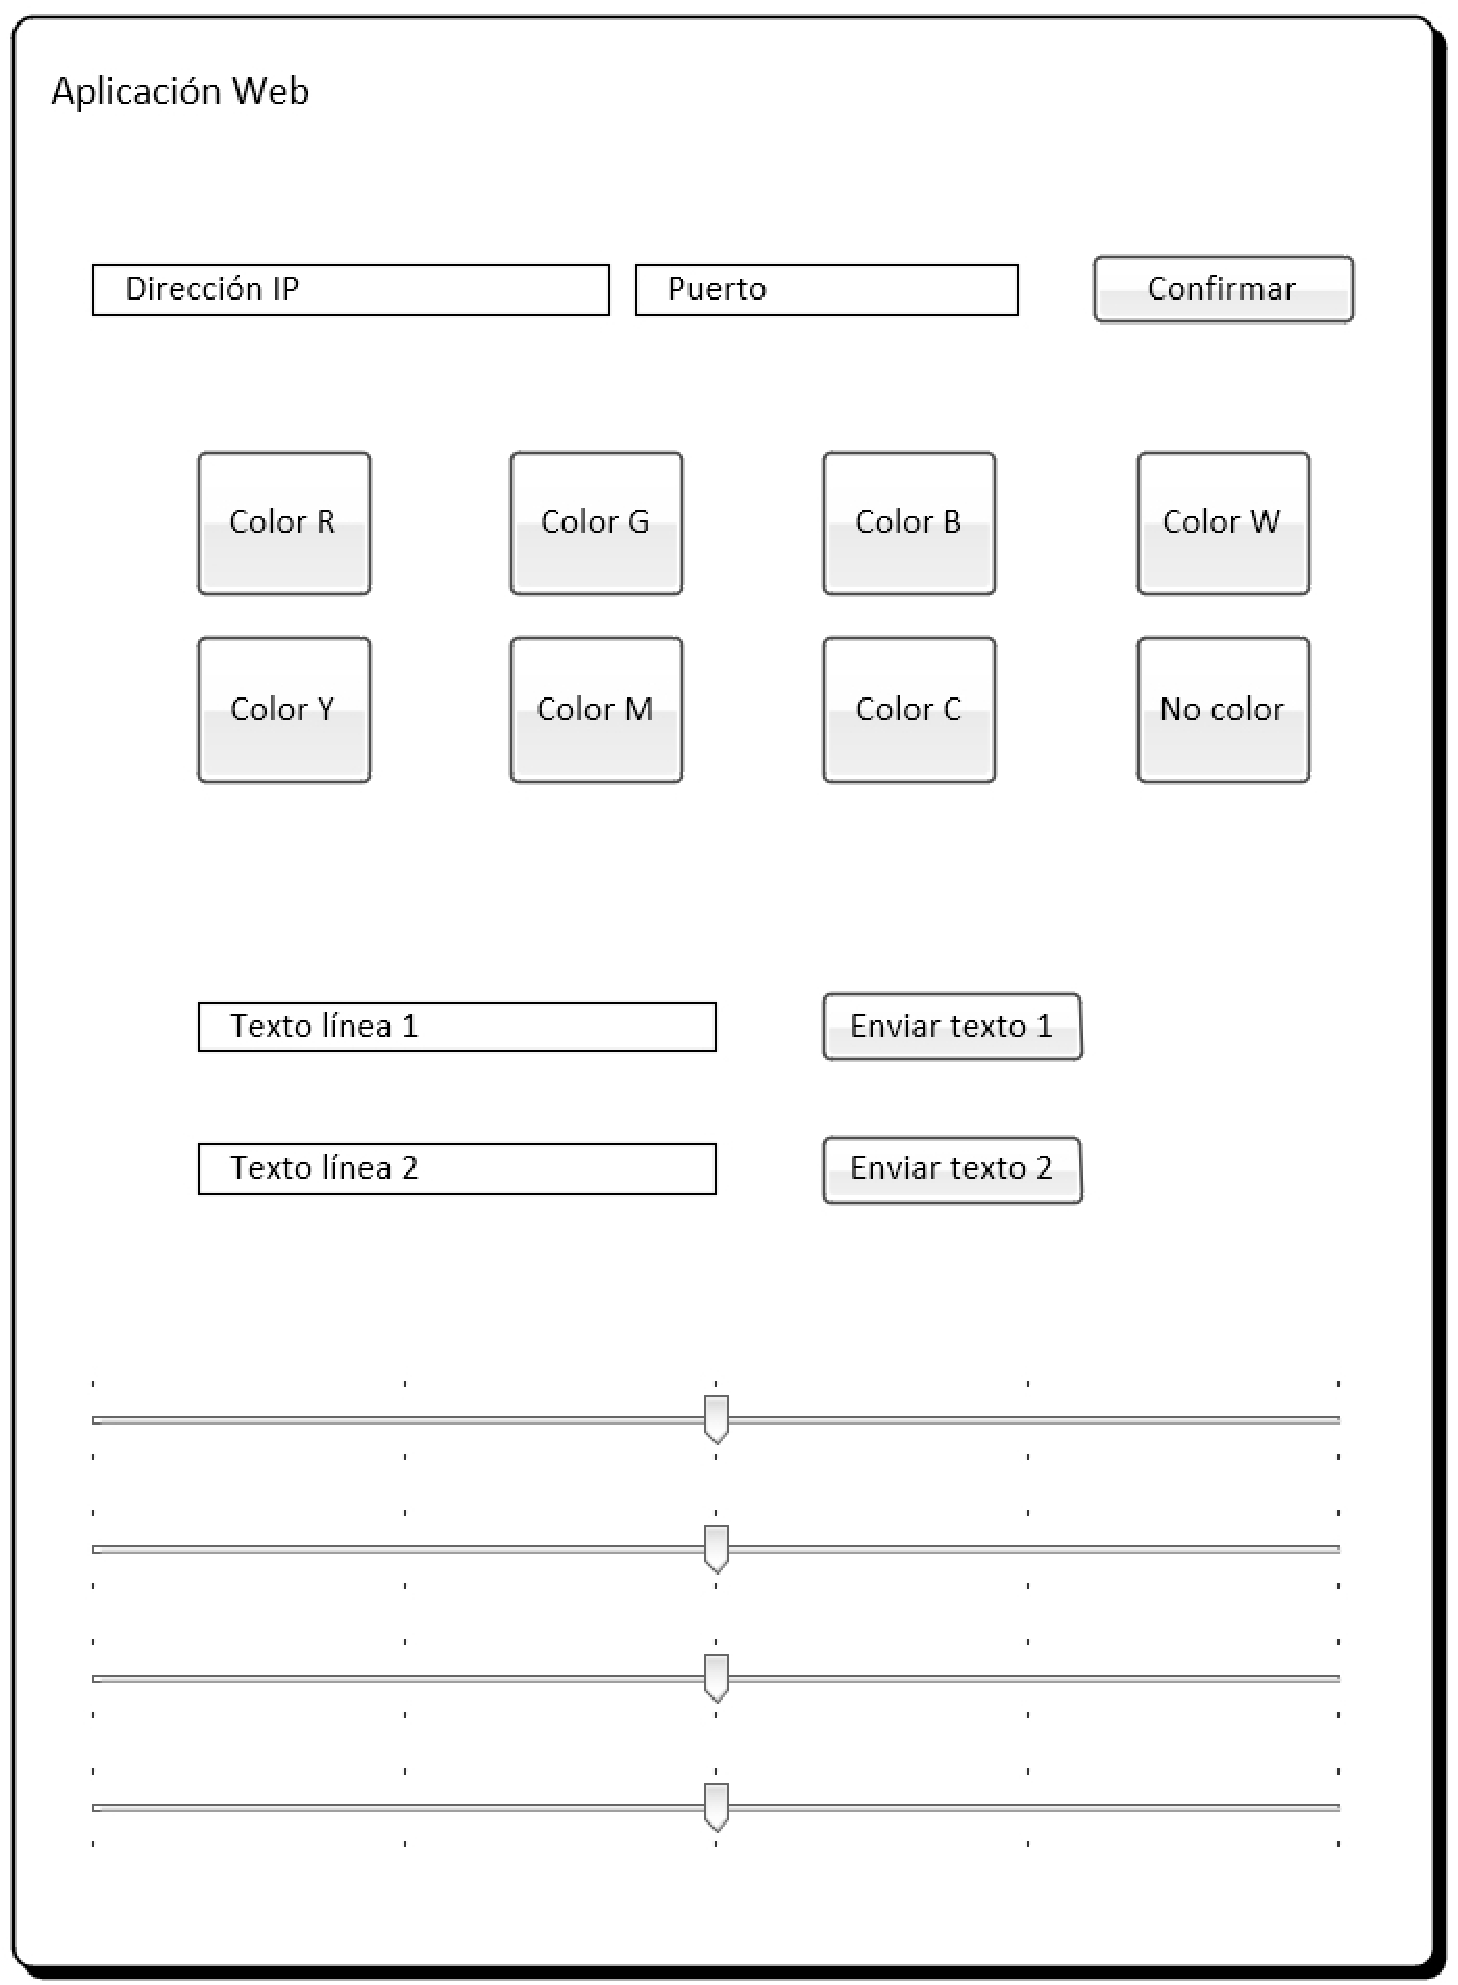
\includegraphics[width=0.55\textheight]{interfaz}
  \caption{Diseño de la interfaz} \label{fig:intefaz}
\end{figure}

\clearpage

\section{Diseño procedimental} \label{sec:design-proc}
El siguiente diagrama muestra las interacciones que se producen entre
los componentes del sistema desde que el usuario solicita una función hasta que
el sistema empotrado la realiza.

\figuraApaisadaSinMarco{0.9}{secuencia}{Diagrama de secuencia}{fig:secuencia}{}
